% Generated by LitigCharts.PublicationFigures. Captions and provenance are sidecars.
\documentclass[10pt,tikz,border=5pt]{standalone}
\usepackage{lmodern}
\usetikzlibrary{patterns,patterns.meta}
\begin{document}
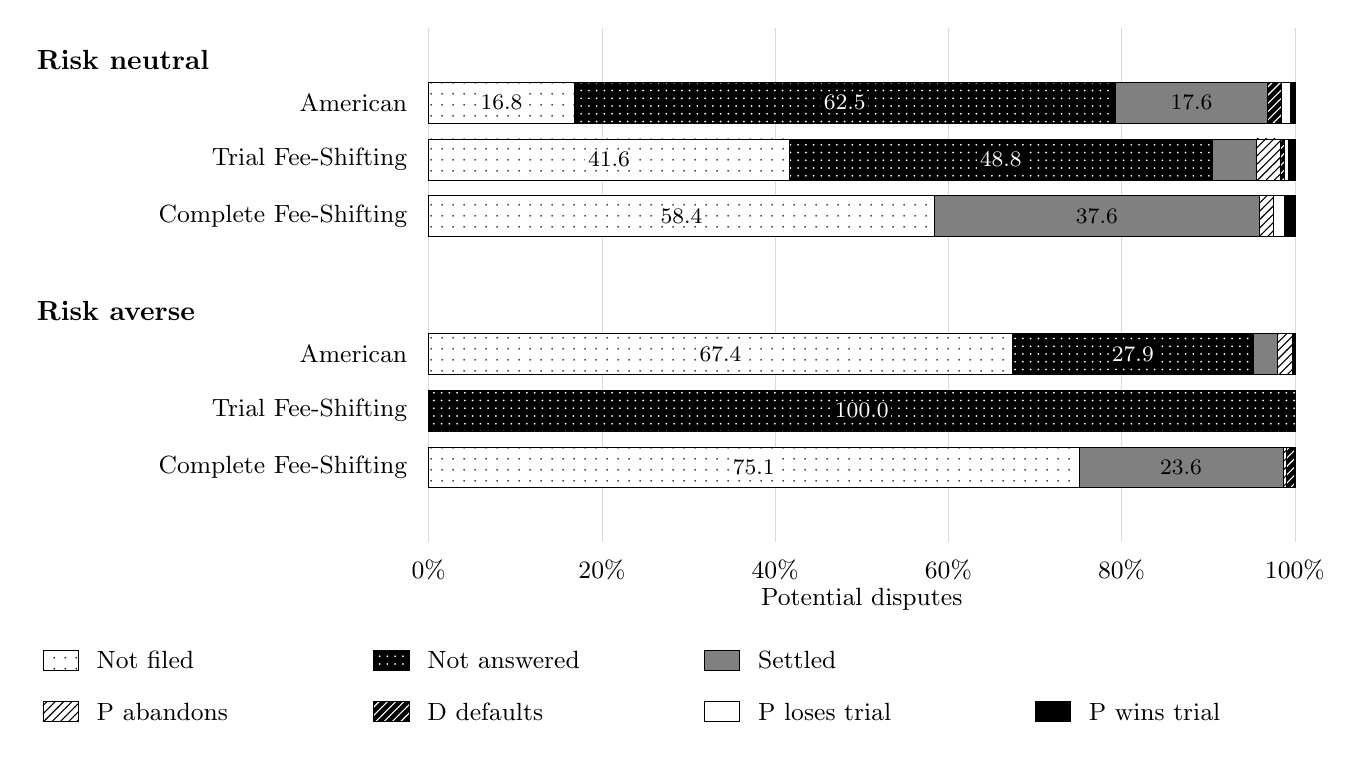
\begin{tikzpicture}[font=\small]\draw[black!15,line width=.2pt] (5.1,.65) -- (5.1,7.18);
\node[anchor=north] at (5.1,.55) {0\%};
\draw[black!15,line width=.2pt] (7.3,.65) -- (7.3,7.18);
\node[anchor=north] at (7.3,.55) {20\%};
\draw[black!15,line width=.2pt] (9.5,.65) -- (9.5,7.18);
\node[anchor=north] at (9.5,.55) {40\%};
\draw[black!15,line width=.2pt] (11.7,.65) -- (11.7,7.18);
\node[anchor=north] at (11.7,.55) {60\%};
\draw[black!15,line width=.2pt] (13.9,.65) -- (13.9,7.18);
\node[anchor=north] at (13.9,.55) {80\%};
\draw[black!15,line width=.2pt] (16.1,.65) -- (16.1,7.18);
\node[anchor=north] at (16.1,.55) {100\%};
\node[anchor=west,font=\bfseries] at (0,6.78) {\mbox{Risk} \mbox{neutral}};
\node[anchor=east] at (4.95,6.23) {American};
\path[preaction={fill=white,draw=none},pattern={Dots[distance=4pt,radius=.35pt]},pattern color=black,draw=black,line width=.25pt] (5.1,5.97) rectangle (6.948011,6.49);
\node[text=black,fill=white,font=\footnotesize,inner sep=1pt] at (6.024006,6.23) {16.8};
\path[preaction={fill=black,draw=none},pattern={Dots[distance=2.8pt,radius=.35pt]},pattern color=white,draw=black,line width=.25pt] (6.948011,5.97) rectangle (13.820525,6.49);
\node[text=white,fill=black,font=\footnotesize,inner sep=1pt] at (10.384268,6.23) {62.5};
\path[fill=black!50,draw=black,line width=.25pt] (13.820525,5.97) rectangle (15.752807,6.49);
\node[text=black,fill=none,font=\footnotesize,inner sep=1pt] at (14.786666,6.23) {17.6};
\path[preaction={fill=black,draw=none},pattern={north east lines},pattern color=white,draw=black,line width=.25pt] (15.752807,5.97) rectangle (15.933945,6.49);
\path[fill=white,draw=black,line width=.25pt] (15.933945,5.97) rectangle (16.047738,6.49);
\path[fill=black,draw=black,line width=.25pt] (16.047738,5.97) rectangle (16.100001,6.49);
\node[anchor=east] at (4.95,5.51) {Trial Fee-Shifting};
\path[preaction={fill=white,draw=none},pattern={Dots[distance=4pt,radius=.35pt]},pattern color=black,draw=black,line width=.25pt] (5.1,5.25) rectangle (9.68007,5.77);
\node[text=black,fill=white,font=\footnotesize,inner sep=1pt] at (7.390035,5.51) {41.6};
\path[preaction={fill=black,draw=none},pattern={Dots[distance=2.8pt,radius=.35pt]},pattern color=white,draw=black,line width=.25pt] (9.68007,5.25) rectangle (15.05181,5.77);
\node[text=white,fill=black,font=\footnotesize,inner sep=1pt] at (12.36594,5.51) {48.8};
\path[fill=black!50,draw=black,line width=.25pt] (15.05181,5.25) rectangle (15.605814,5.77);
\path[preaction={fill=white,draw=none},pattern={north east lines},pattern color=black,draw=black,line width=.25pt] (15.605814,5.25) rectangle (15.92197,5.77);
\path[preaction={fill=black,draw=none},pattern={north east lines},pattern color=white,draw=black,line width=.25pt] (15.92197,5.25) rectangle (15.963929,5.77);
\path[fill=white,draw=black,line width=.25pt] (15.963929,5.25) rectangle (16.021607,5.77);
\path[fill=black,draw=black,line width=.25pt] (16.021607,5.25) rectangle (16.100005,5.77);
\node[anchor=east] at (4.95,4.79) {Complete Fee-Shifting};
\path[preaction={fill=white,draw=none},pattern={Dots[distance=4pt,radius=.35pt]},pattern color=black,draw=black,line width=.25pt] (5.1,4.53) rectangle (11.51993,5.05);
\node[text=black,fill=white,font=\footnotesize,inner sep=1pt] at (8.309965,4.79) {58.4};
\path[fill=black!50,draw=black,line width=.25pt] (11.51993,4.53) rectangle (15.652322,5.05);
\node[text=black,fill=none,font=\footnotesize,inner sep=1pt] at (13.586126,4.79) {37.6};
\path[preaction={fill=white,draw=none},pattern={north east lines},pattern color=black,draw=black,line width=.25pt] (15.652322,4.53) rectangle (15.822109,5.05);
\path[fill=white,draw=black,line width=.25pt] (15.822109,4.53) rectangle (15.961049,5.05);
\path[fill=black,draw=black,line width=.25pt] (15.961049,4.53) rectangle (16.099996,5.05);
\node[anchor=west,font=\bfseries] at (0,3.59) {\mbox{Risk} \mbox{averse}};
\node[anchor=east] at (4.95,3.04) {American};
\path[preaction={fill=white,draw=none},pattern={Dots[distance=4pt,radius=.35pt]},pattern color=black,draw=black,line width=.25pt] (5.1,2.78) rectangle (12.50971,3.3);
\node[text=black,fill=white,font=\footnotesize,inner sep=1pt] at (8.804855,3.04) {67.4};
\path[preaction={fill=black,draw=none},pattern={Dots[distance=2.8pt,radius=.35pt]},pattern color=white,draw=black,line width=.25pt] (12.50971,2.78) rectangle (15.576367,3.3);
\node[text=white,fill=black,font=\footnotesize,inner sep=1pt] at (14.043039,3.04) {27.9};
\path[fill=black!50,draw=black,line width=.25pt] (15.576367,2.78) rectangle (15.873941,3.3);
\path[preaction={fill=white,draw=none},pattern={north east lines},pattern color=black,draw=black,line width=.25pt] (15.873941,2.78) rectangle (16.072699,3.3);
\path[preaction={fill=black,draw=none},pattern={north east lines},pattern color=white,draw=black,line width=.25pt] (16.072699,2.78) rectangle (16.085469,3.3);
\path[fill=white,draw=black,line width=.25pt] (16.085469,2.78) rectangle (16.089864,3.3);
\path[fill=black,draw=black,line width=.25pt] (16.089864,2.78) rectangle (16.100004,3.3);
\node[anchor=east] at (4.95,2.32) {Trial Fee-Shifting};
\path[preaction={fill=black,draw=none},pattern={Dots[distance=2.8pt,radius=.35pt]},pattern color=white,draw=black,line width=.25pt] (5.1,2.06) rectangle (16.1,2.58);
\node[text=white,fill=black,font=\footnotesize,inner sep=1pt] at (10.6,2.32) {100.0};
\node[anchor=east] at (4.95,1.6) {Complete Fee-Shifting};
\path[preaction={fill=white,draw=none},pattern={Dots[distance=4pt,radius=.35pt]},pattern color=black,draw=black,line width=.25pt] (5.1,1.34) rectangle (13.35682,1.86);
\node[text=black,fill=white,font=\footnotesize,inner sep=1pt] at (9.22841,1.6) {75.1};
\path[fill=black!50,draw=black,line width=.25pt] (13.35682,1.34) rectangle (15.949454,1.86);
\node[text=black,fill=none,font=\footnotesize,inner sep=1pt] at (14.653137,1.6) {23.6};
\path[preaction={fill=white,draw=none},pattern={north east lines},pattern color=black,draw=black,line width=.25pt] (15.949454,1.34) rectangle (15.987047,1.86);
\path[preaction={fill=black,draw=none},pattern={north east lines},pattern color=white,draw=black,line width=.25pt] (15.987047,1.34) rectangle (16.098583,1.86);
\path[fill=white,draw=black,line width=.25pt] (16.098583,1.34) rectangle (16.099292,1.86);
\path[fill=black,draw=black,line width=.25pt] (16.099292,1.34) rectangle (16.100001,1.86);
\node at (10.6,-.08) {Potential disputes};
\path[preaction={fill=white,draw=none},pattern={Dots[distance=4pt,radius=.35pt]},pattern color=black,draw=black,line width=.25pt] (0.2,-0.98) rectangle (0.65,-0.72);
\node[anchor=west] at (0.76,-0.85) {Not filed};
\path[preaction={fill=black,draw=none},pattern={Dots[distance=2.8pt,radius=.35pt]},pattern color=white,draw=black,line width=.25pt] (4.4,-0.98) rectangle (4.85,-0.72);
\node[anchor=west] at (4.96,-0.85) {Not answered};
\path[fill=black!50,draw=black,line width=.25pt] (8.6,-0.98) rectangle (9.05,-0.72);
\node[anchor=west] at (9.16,-0.85) {Settled};
\path[preaction={fill=white,draw=none},pattern={north east lines},pattern color=black,draw=black,line width=.25pt] (0.2,-1.63) rectangle (0.65,-1.37);
\node[anchor=west] at (0.76,-1.5) {P abandons};
\path[preaction={fill=black,draw=none},pattern={north east lines},pattern color=white,draw=black,line width=.25pt] (4.4,-1.63) rectangle (4.85,-1.37);
\node[anchor=west] at (4.96,-1.5) {D defaults};
\path[fill=white,draw=black,line width=.25pt] (8.6,-1.63) rectangle (9.05,-1.37);
\node[anchor=west] at (9.16,-1.5) {P loses trial};
\path[fill=black,draw=black,line width=.25pt] (12.8,-1.63) rectangle (13.25,-1.37);
\node[anchor=west] at (13.36,-1.5) {P wins trial};
\end{tikzpicture}
\end{document}
